\documentclass{article}
\renewcommand{\reals}{\mathbb{R}}

% If you're new to LaTeX, here's some short tutorials:
% https://www.overleaf.com/learn/latex/Learn_LaTeX_in_30_minutes
% https://en.wikibooks.org/wiki/LaTeX/Basics

% Formatting
\usepackage[utf8]{inputenc}
\usepackage[margin=1in]{geometry}
\usepackage[titletoc,title]{appendix}
\usepackage{pdfpages}
\usepackage{placeins}

% Math
% https://www.overleaf.com/learn/latex/Mathematical_expressions
% https://en.wikibooks.org/wiki/LaTeX/Mathematics
\usepackage{amsmath,amsfonts,amssymb,mathtools}

% Images
% https://www.overleaf.com/learn/latex/Inserting_Images
% https://en.wikibooks.org/wiki/LaTeX/Floats,_Figures_and_Captions
\usepackage{graphicx,float}

% Tables
% https://www.overleaf.com/learn/latex/Tables
% https://en.wikibooks.org/wiki/LaTeX/Tables

% Code syntax highlighting
% https://www.overleaf.com/learn/latex/Code_Highlighting_with_minted
\usepackage{minted}
\usemintedstyle{borland}

% References
% https://www.overleaf.com/learn/latex/Bibliography_management_in_LaTeX
% https://en.wikibooks.org/wiki/LaTeX/Bibliography_Management
\usepackage{biblatex}
\addbibresource{references.bib}

% Title content
\title{Coding Project - Compressed Sensing }
\author{Wonnetz Phanthavong}
\date{November 17, 2020}

\begin{document}

\maketitle

% Introduction and Overview
\section{Introduction and Overview}
Compressed Sensing involves reconstructing a sparse signal $x \in \reals^{n}$. This takes the form $b = Ax$, where $b \in \reals^{n}$ is our sampled vector and $A \in \reals^{m\text{ x } n}$ is our predefined sampling matrix. Note, $A$ can be populated with either Gaussian or Bernoulli entries, the key to $A$ is to have some randomness built into it \cite{brunton2019data}. In this case we shall use Gaussian entries to populate our sampling matrix $A$. It has been shown that we can solve the Compressed Sensing problem through
$$
\min_{x} \{\|x\|_{0}\} \quad \text{subject to } Ax = b
$$
However, this is a NP hard problem, which means that this problem is difficult to compute. Thus, we shall instead opt to solve the  below problem, which still has a high probability of reconstructing $x$ \cite{candes2006robust}. 
$$
\min_{x} \{ \|x\|_{1} + \frac{\lambda}{2\tau}\|Ax-b\|_{2}^{2} \} \quad \textbf{(1)}
$$
A natural question here is, "Why not use the L2 norm $\|\cdot\|_{2}$"? Observe that for our vector $x$, if we were to use the L2 norm to minimize the problem, then there is a high probability to recover a non-sparse solution \cite{brunton2019data}. The L1 norm, $\|\cdot\|_{1}$, allows us to reconstruct a solution that is more likely to be sparse. Intuitively, one can observe the geometry of the L1 norm and L2 norm to see this difference. Supposing that we are working in $\reals^{2}$ and we have sampled a vector. Minimizing the L1 norm gives us a rhombus that grows to intersect the vector on either the x-axis or y-axis, where as minimizing the L2 norm gives us a circle that grows to intersect the vector at some point that is a combination of both x and y. Hence, minimizing the L1 norm gives us a sparse vector, where as minimizing the L2 norm gives us a non-sparse vector. \\
\ \\
For notation sake, sometimes we will use the following, let $\phi(x) = \|x\|_{1}$ and $f(x) = \frac{\lambda}{2}\|Ax -b\|_{2}^{2}$. Then we will have, 
$$
\min_{x} \{ \phi(x) + f(x)\}
$$
Note, $\lambda$ is a user chosen parameter and $\tau \in (0, \frac{2}{L})$, where L is the Lipschitz constant of $\nabla f$, i.e. $L = \lambda\|A^{T}A\|_{2}$. Here we shall use $\lambda = 2$ and $\tau = \frac{1}{L}$.
First we shall observe what happens when we attempt to solve \textbf{(1)} through the Proximal Gradient Descent and then Tseng's Accelerated Proximal Gradient Method. 

% Proximal Operator
\section{Regular Proximal Operator Method}
First we shall describe how to compute the Proximal Operator on the Gradient Descent step, shown below, 
$$
prox_{\tau \phi} := argmin_{x \in \reals^{n}} \{ \phi(x) + \frac{1}{2}\| x -z \|^{2} \}
$$
To figure this out, we shall first work out the Proximal Operator of the Absolute Value function $| \cdot |$, below
$$
prox_{\tau |\cdot|}(x) = argmin_{x \in \reals^{n}} \{ |x| + \frac{1}{2\tau}|x-z|^{2} \}
$$
As we are working with absolute values, naturally, let us consider two different cases. The case when $x \geq 0$ and the case when $x \leq 0$. \\
\ \\
\textbf{Case 1: } $x \geq 0$ \\
Observe that this reduces the Proximal Operator to
$$
prox_{\tau |\cdot|}(x) = argmin_{x \in \reals^{n}} \{ x + \frac{1}{2\tau}(x-z)^{2} \}
$$
Through some Calculus 1, we find that the minimizer for the above will be given as 
$$
x = z -\tau
$$
Recall that we restricted our $x$ to be $x \geq 0$, hence we have one more condition. \\
Hence, $x \geq 0 \implies z - \tau \geq 0 \implies z \geq \tau$, then for $z < \tau$ we shall then set $x = 0$. \\
Hence, the closed form formula will be given as
$$
prox_{\tau |\cdot|}(x) = argmin_{x \in \reals^{n}} \{ x + \frac{1}{2\tau}(x-z)^{2} \} = \left\{\begin{array}{l}
x = z - \tau \text{ for } z \geq \tau \\
x = 0 \text{ for } z < \tau
\end{array}\right.
$$
\ \\
\textbf{Case 2: } $x \leq 0$ \\
Similar to how we handled Case 1, we shall arrive at 
$$
prox_{\tau |\cdot|}(x) = argmin_{x \in \reals^{n}} \{ -x + \frac{1}{2\tau}(x-z)^{2} \} = 
\left\{\begin{array}{l}
x = z + \tau \text{ for } z \leq -\tau \\
x = 0 \text{ for } z > \tau
\end{array}\right.
$$
\ \\
\noindent
Putting Case 1 and Case 2 together gives us
$$
prox_{\tau |\cdot|}(x) = argmin_{x \in \reals^{n}} \{ |x| + \frac{1}{2\tau}|x-z|^{2} \} = 
\left\{\begin{array}{l}
x = z - \tau \text{ for } z \geq \tau \\
x = z + \tau \text{ for } z \leq -\tau \\
x = 0 \text{ for } -\tau > z > \tau
\end{array}\right.
$$

Now that we have figured out the Proximal Operator on the Absolute Value function, let us see how this relates to the main problem at hand. \\
\ \\
Observe that for, 
$$
prox_{\tau \phi} := argmin_{x \in \reals^{n}} \{ \|x\|_{1} + \frac{\lambda}{2}\| x -z \|^{2}_{2} \}
$$
we can view this as minimizing each vector component for $\|x\|_{1}$ and $\frac{\lambda}{2}\|x-z\|_{2}^{2}$. Which means that we can perform the Proximal Operator on the Absolute Value function from $i \rightarrow n$ for $|x_{k}^{(i)}|$ and $\frac{\lambda}{2}(x_{k}^{(i)} - z_{k}^{(i)})^{2}$ where $k$ represents the iteration number and $i$ represents the $i^{th}$ component of  the vectors. 





% Accelerated Proximal Gradient Method
\section{Accelerated Proximal Gradient Method}
Now we shall figure out how to implement the Accelerated Proximal Gradient Method \cite{tseng2008accelerated}. To reiterate the problem, the nonsmooth convex optimization problem that we are working with is given as
$$
\min_{x} \{ f(x) + \phi(x) \}
$$
In light of Nesterov extending his third method with this Bregman function, we shall choose the same one.\\
Let $D(x,y) = \frac{1}{2}\| x-y \|^{2}_{2}$ be our Bregman function \cite{nesterov2007dual}.\\

The key step here involves figuring out how to implement 
$$
z_{k+1} = argmin_{x \in \reals^{n}}\{ l_{f}(x;y_{k}) + \theta_{k}LD(x, z_{k}) \}
$$
\ \\
Where,
$$
l_{f}(x;y) := f(y) + \langle \nabla f(y), x-y \rangle + \phi(x)
$$
$$
\theta_{0} = 1 \text{ and } \theta_{k} = \frac{2}{k + 2}
$$
$$
D(x,y) = \frac{1}{2}\|x-y\|_{2}^{2}
$$
Note, $f(x),\phi(x), L$ are chosen as in \textbf{Section 2}. \\
Plugging everything in, we have
$$
z_{k+1} = argmin_{x \in \reals^{n}} \left\{\frac{\lambda}{2}\|Ay_{k}-b\|_{2}^{2} + \langle \nabla f(y_{k}), x - y_{k} \rangle + \|x\|_{1} + \theta_{k}\frac{L}{2}\|x-z_{k}\|_{2}^{2} \right\}
$$
Let us focus primarily on the 1-Dimensional case of the above, given below
$$
argmin_{x \in \reals} \left\{\frac{\lambda}{2}((Ay_{k})^{(i)}-b^{(i)})^{2} + \langle \nabla f(y_{k})^{(i)}, x - y_{k}^{(i)} \rangle + |x| + \theta_{k}\frac{L}{2}(x-z_{k}^{(i)})^{2}\right\}
$$
Familiarly, the above looks similar to the Proximal Operator case! \\
Hence, by observing the cases when $x \leq 0$ and $x \geq 0$, we find the closed form of the 1-Dimensional case to be given below
\scriptsize
$$
argmin_{x \in \reals} \left\{\frac{\lambda}{2}((Ay_{k})^{(i)}-b^{(i)})^{2} + \langle \nabla f(y_{k})^{(i)}, x - y_{k}^{(i)} \rangle + |x| + \theta_{k}\frac{L}{2}(x-z_{k}^{(i)})^{2}\right\} = 
\left\{\begin{array}{l}
x^{(i)} = z^{(i)} - \frac{1 + \nabla f(y_{k})^{(i)}}{\theta_{k}L} \text{ for } z \geq \frac{1 + \nabla f(y_{k})^{(i)}}{\theta_{k}L} \\
\\
x^{(i)} = z^{(i)} + \frac{1 - \nabla f(y_{k})^{(i)}}{\theta_{k}L} \text{ for } z \leq \frac{\nabla f(y_{k})^{(i)} - 1}{\theta_{k}L} \\
\\
x^{(i)} = 0 \text{ for } \frac{1 + \nabla f(y_{k})^{(i)}}{\theta_{k}L} < z < \frac{\nabla f(y_{k})^{(i)} - 1}{\theta_{k}L}
\end{array}\right.
$$
\normalsize
Finally, for the case of $x \in \reals^{n}$, we have
$$
argmin_{x \in \reals^{n}}\left\{\frac{\lambda}{2}\|Ay_{k}-b\|_{2}^{2} + \langle \nabla f(y_{k}), x - y_{k} \rangle + \|x\|_{1} + \theta_{k}\frac{L}{2}\|x-z_{k}\|_{2}^{2} \right\} = 
\left\{\begin{array}{l}
x = z - \frac{1 + \nabla f(y_{k})}{\theta_{k}L} \text{ for } z \geq \frac{1 + \nabla f(y_{k})}{\theta_{k}L} \\
\\
x = z + \frac{1 - \nabla f(y_{k})}{\theta_{k}L} \text{ for } z \leq \frac{\nabla f(y_{k}) - 1}{\theta_{k}L} \\
\\
x = 0 \text{ for } \frac{1 + \nabla f(y_{k})}{\theta_{k}L} < z < \frac{\nabla f(y_{k}) - 1}{\theta_{k}L}
\end{array}\right.
$$

% Summary and Conclusions
\section{Summary and Conclusions}
Now let us look at the results of both of these algorithms! Both algorithms converge to the unique solution for \textbf{(1)}, $\hat{x}$. Note, the solution is unique, due to the convexity of \textbf{(1)}. This can be seen from graphing the 1-Dimensional case of \textbf{(1)}. Unsurprisingly, we see that the Accelerated Proximal Gradient Method converges faster than the Regular Proximal Gradient Method.  For a randomly generated $x_{0}, z_{0} \in \reals^{n}$ with normally distributed values, we will see the following graphs,

\begin{figure}[hbp]
    \centering
    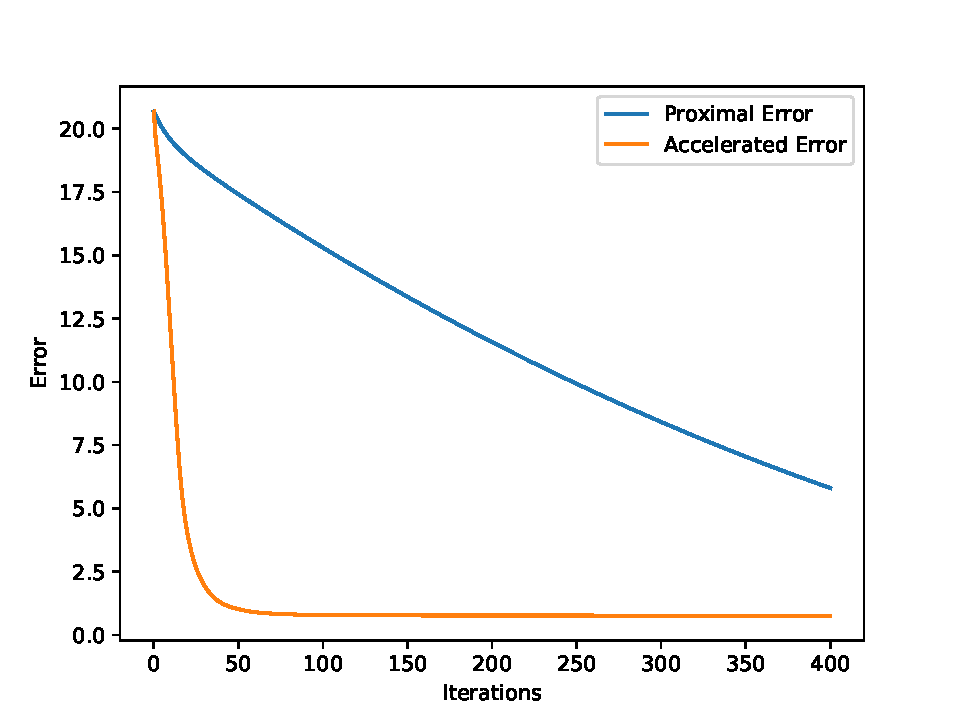
\includegraphics[width=120mm]{Error.pdf}
    \caption{Error between Proximal Method and the Accelerated Proximal Method}
    \label{fig:fig 1}
\end{figure}

\begin{figure}[hbp]
    \centering
    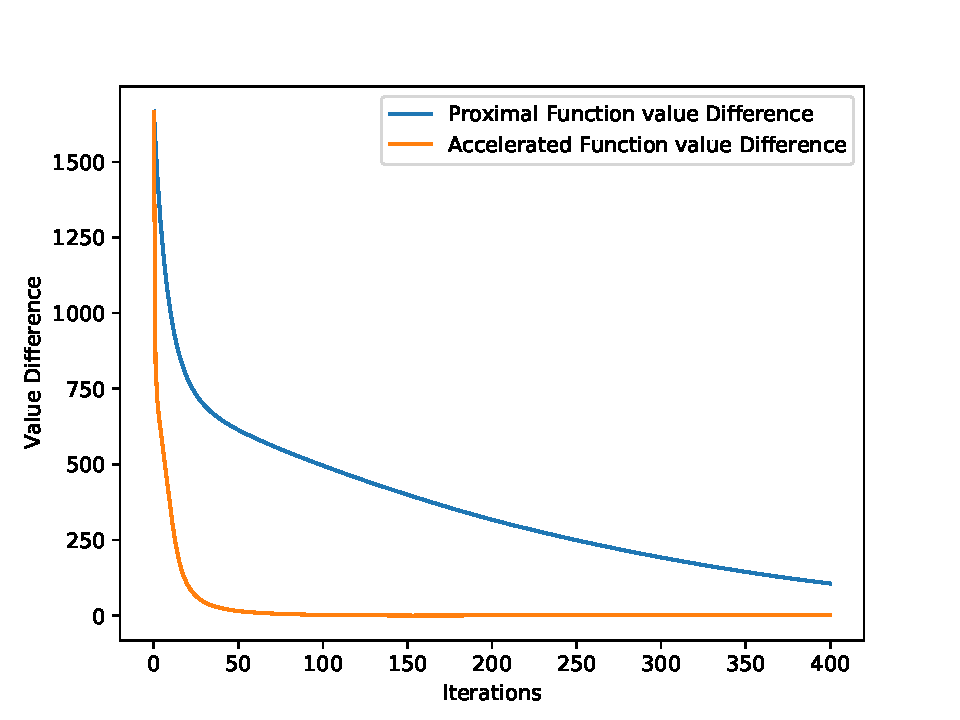
\includegraphics[width=120mm]{Function Difference.pdf}
    \caption{Difference in Function Values for the Proximal Method and the Accelerated Proximal Method}
    \label{fig:my_label}
\end{figure}

\newpage

\section{Final Remarks}
\begin{enumerate}
    \item I found that in the plot of $f(x_{k}) - f(\hat{x})$, for the Proximal Gradient Method, it did not have a convergence rate of $O(\frac{1}{k})$, but rather that it converged at a rate of $O(\frac{1}{\sqrt{k}})$. 
    \item I decided to withhold on coding Section 3 for now. Perhaps I will come back to it during Thanksgiving Break or after Finals. I left off with trying to figure out how to create either an Orthonormal Haar matrix or an Orthonormal Fourier matrix to transform a non-sparse vector to a sparse vector. I opted to construct these matrices instead of using Python's library, because the Pywt package and Fast Fourier Transform function returned a vector that had half the length I desired. I was not sure how to proceed with this, so I'll look into it at a later date. 
    \item Lastly, there are a couple formatting nuances that I wanted to rework with my Python code. The aesthetics of the graphs could be improved and the code itself is structured a bit odd. I see that Nathan had a main environment that he ran his python code and he kept his algorithms in separate python files. In the future I will follow this technique. That way is a bit neater and I think it's standard.
\end{enumerate}


% References
\printbibliography



\end{document}
